\documentclass[border=5pt]{standalone}
\usepackage{tikz}
\usepackage{xcolor}
\usetikzlibrary{calc,shadows.blur}

% J8 - Yellow rectangular block
\begin{document}
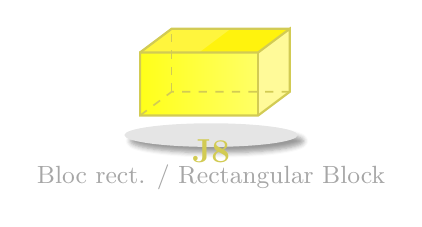
\begin{tikzpicture}

% Shadow
\fill[gray!20,blur shadow={shadow blur steps=5}] (0.9,-0.25) ellipse (1.1 and 0.15);

% Back face
\fill[yellow!30] (0.4,0.3) -- (1.9,0.3) -- (1.9,1.1) -- (0.4,1.1) -- cycle;

% Left face (side)
\fill[yellow!50] (0.0,0.0) -- (0.4,0.3) -- (0.4,1.1) -- (0.0,0.8) -- cycle;

% Front face (main)
\fill[left color=yellow!80, right color=yellow!50]
  (0.0,0.0) -- (1.5,0.0) -- (1.9,0.3) -- (0.4,0.3) -- cycle;

% Isometric top view
\fill[yellow!80,opacity=0.9] (0.0,0.8) -- (1.5,0.8) -- (1.9,1.1) -- (0.4,1.1) -- cycle;

% Front-top connection
\fill[left color=yellow!90, right color=yellow!60]
  (0.0,0.0) -- (1.5,0.0) -- (1.5,0.8) -- (0.0,0.8) -- cycle;

% Right face
\fill[yellow!40] (1.5,0.0) -- (1.9,0.3) -- (1.9,1.1) -- (1.5,0.8) -- cycle;

% Top face
\fill[yellow!95] (0.0,0.8) -- (1.5,0.8) -- (1.9,1.1) -- (0.4,1.1) -- cycle;

% Highlight on top
\fill[white,opacity=0.2] (0.0,0.8) -- (0.75,0.8) -- (1.15,1.1) -- (0.4,1.1) -- cycle;

% Edges
\draw[yellow!60!gray, line width=0.8pt]
  (0.0,0.0) -- (1.5,0.0) -- (1.9,0.3) -- (1.9,1.1) -- (1.5,0.8)
  -- (0.0,0.8) -- cycle;
\draw[yellow!60!gray, line width=0.8pt]
  (0.0,0.8) -- (0.4,1.1) -- (1.9,1.1);
\draw[yellow!60!gray, line width=0.8pt]
  (1.5,0.0) -- (1.5,0.8);
\draw[yellow!60!gray, line width=0.6pt, dashed]
  (0.0,0.0) -- (0.4,0.3) -- (1.9,0.3);
\draw[yellow!60!gray, line width=0.6pt, dashed]
  (0.4,0.3) -- (0.4,1.1);

% Label
\node[font=\bfseries\large, text=yellow!60!gray] at (0.9,-0.45) {J8};
\node[font=\small, text=gray!70] at (0.9,-0.78) {Bloc rect. / Rectangular Block};

\end{tikzpicture}
\end{document}
